\documentclass{article}
\usepackage[utf8]{inputenc}

\title{Tugas Harian I}
\author{ Fadila }
\date{26 February 2019}

\usepackage{natbib}
\usepackage{graphicx}

\begin{document}

\maketitle

\section{Fadila/1164072}
\subsection{Teori}
Penyelesaian Tugas Harian 3 ( No. 1-7 )
\begin{enumerate}
\item Binary Classification Dan Ilustrasi Gambarnya
\begin{itemize}
\item Pengertian Binary Classification / Klasifikasi Biner:
\par Klasifikasi biner atau binomial merupakan tugas untuk mengklasifikasikan elemen-elemen dari himpunan tertentu ke dalam dua kelompok (memprediksi kelompok mana yang masing-masing dimiliki) berdasarkan aturan klasifikasi.
\item Ilustrasi Gambar Binary Classification :
\par

\begin{figure}[ht]
\centering
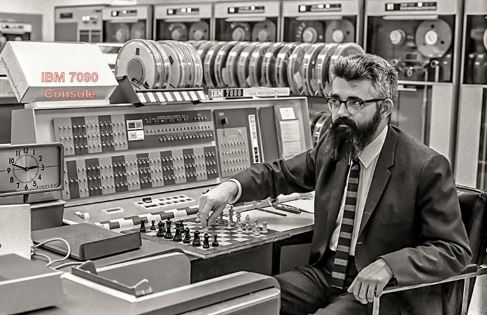
\includegraphics[scale=0.5]{figures/contoh.jpg}
\caption{capturing}
\label{contoh}
\end{figure}

\par
\end{itemize}
\item Supervised Learning, Unsupervised Learning, Clustering Dan Ilustrasi Gambar
\begin{itemize}
\item Pengertian Supervised Learning :
\par Sebuah pendekatan dimana terdapat data yang dilatih dan ditargetkan. Leih singkatnya supervised learning memiliki kategori sehingga tujuan dan outputnya jelas.
\par

\begin{figure}[ht]
\centering
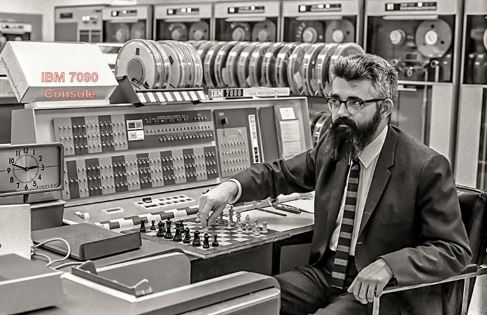
\includegraphics[scale=0.5]{figures/contoh.jpg}
\caption{capturing}
\label{contoh}
\end{figure}

\par
\item Pengertian Unsupervised Learning :
\par Tidak memiliki data latih, sehingga dari data yang tersebut kita bisa mengelompokkannya ke berbagai kelompok 2 seterusnya. Dengan lebih singkatnya ialah unsupervised learning tidak memiliki kategori.
\par

\begin{figure}[ht]
\centering
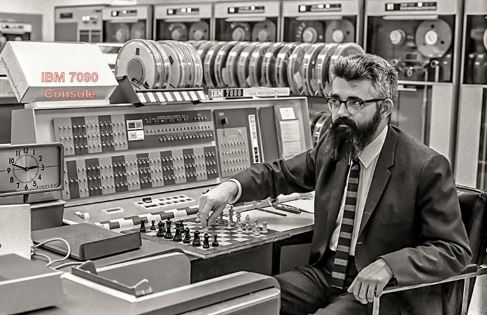
\includegraphics[scale=0.5]{figures/contoh.jpg}
\caption{capturing}
\label{contoh}
\end{figure}

\par
\item Pengertian Unsupervised Learning :
\par Metode pengelompokan data. Clustering juga merupakan proses partisi satu set objek data ke dalam himpunan bagian yang disebut dengan cluster. Objek dalam cluster tersebut memiliki kemiripan karakteristik antar satu sama lain.
\par

\begin{figure}[ht]
\centering
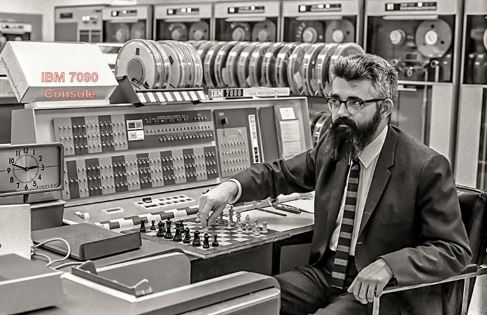
\includegraphics[scale=0.5]{figures/contoh.jpg}
\caption{capturing}
\label{contoh}
\end{figure}

\par
\end{itemize}
\item Evaluasi, Akurasi Dan Ilustrasi Gambar
\begin{itemize}
\item Pengertian Evaluasi
\par Evaluasi digunakan untuk memeriksa/memastikan dan mengevaluasi model dalam bekerja ( seberapa baik ) dengan mengukur keakuratannya. Kita juga dapat menanalisis kesalahan yang dibuat pada model yang dijalankan, tingkat kebingungan dan menggunakan matriks kebingunan.
\par

\begin{figure}[ht]
\centering
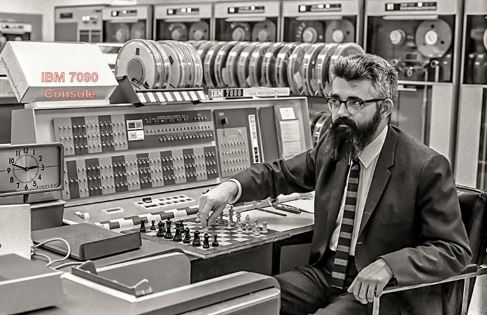
\includegraphics[scale=0.5]{figures/contoh.jpg}
\caption{capturing}
\label{contoh}
\end{figure}

\par
\item Pengertian Akurasi
\par Accuracy akan didefinisikan sebagai presentasi kasus yang diklasifikasikan dengan benar. Accuracy lebih jelasnya adalah perbandingan kasus yang diidentifikasi benar dengan jumlah semua kasus
 \par Rumus dari accuracy= (a+c)/(a+b+c+d)
\par

\begin{figure}[ht]
\centering
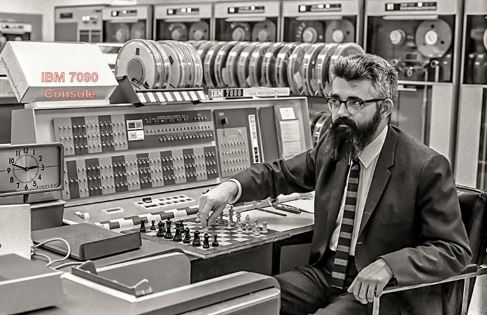
\includegraphics[scale=0.5]{figures/contoh.jpg}
\caption{capturing}
\label{contoh}
\end{figure}

\par
\end{itemize}